\chapter{State-of-the-Art}
Crowd motion analysis deals with a combination of computer vision, Image processing and machine 
learning techniques. This section provides in depth knowledge of related work and state of the art 
techniques by explaining the recent and ground braking scientific papers in this field. More specifically 
the motivation introduction and the techniques used in these papers.
\section{Crowd analysis by using optical flow}
The papers ~\cite{santoro2010crowd} ~\cite{rosandic2019crowd} gives a generic and very efficient way 
of tracking the crowd motion in the videos. As shown in the figure \ref{fig:opticaldataflow} below, the 
process of crowd tracking is done in 4 steps. 
\begin{figure}[tb]
	\center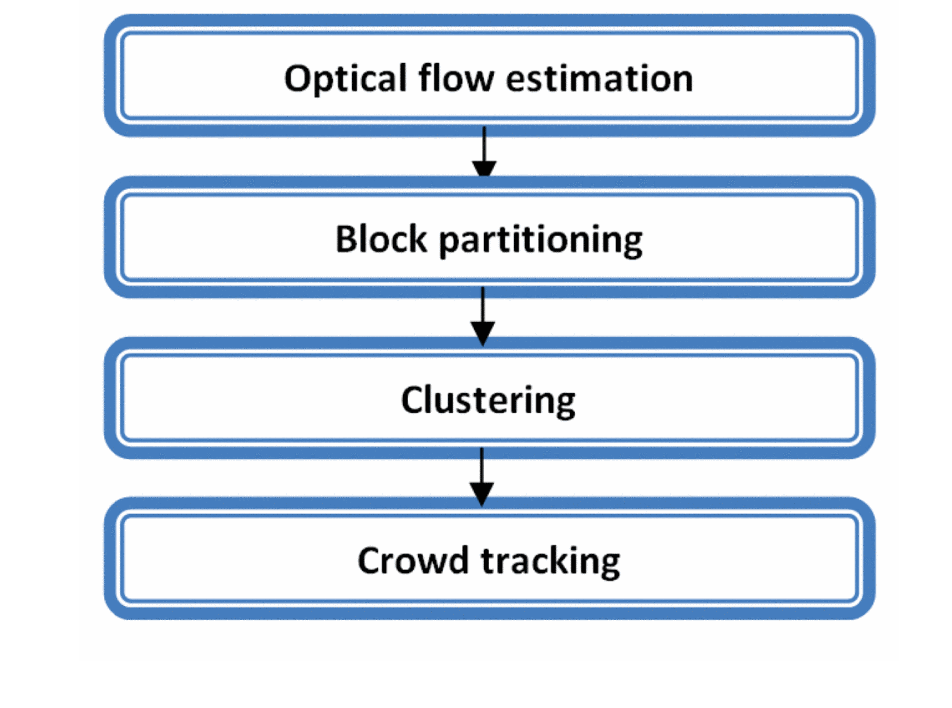
\includegraphics[width=0.6\textwidth]{Opticalflowdataflow.png}
	\caption{Data Flow Diagram}
	\label{fig:opticaldataflow}
\end{figure}
KLT feature tracker is used to do the optical flow estimation.KLT feature tracker is the combination of Shi-
Tomasi corner detection and the famous Lucas Kanade optical flow algorithm. Shi-Tomasi corner 
detection technique is used to identify the interesting corners of the frame. A section of surrounding 
pixels of these points are also added to the tracking. This step is followed by tracking the points in the consequent frames. The tracking is done with the help of Lucas Kanade algorithm. In addition to the change in the points, magnitude and the angle of the vector is also calculated at this point of time.

Now that all the vectors are derived from frame fk and fk+1, block partitioning is done on the whole frame. The frame is divided in to multiple blocks and the vectors in the specific blocks are clustered based on the angle and magnitude. This clustering is done with the help of DBSCAN algorithm. All the points which are considered to be one group are marked with single vector. Any person leaving the crowd or joining the crowd is considered as separate or single block accordingly. The result of this paper are shown in the figure \ref{fig:opticalflowresult}. The person behind the crowd is considered as separate group and the tracking is done multiple times to get the flow.
\begin{figure}[tb]
	\center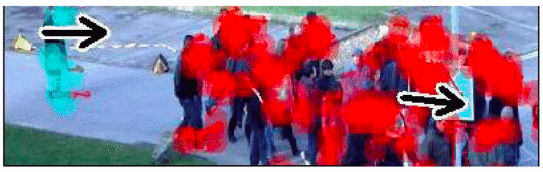
\includegraphics[width=0.6\textwidth]{opticalflowresult.png}
	\caption{Density based partitioning and crowd tracking}
	\label{fig:opticalflowresult}
\end{figure}

The paper ~\cite{4629878} is an interesting use of optical flow to detect the dominant motion in the crowded scenes. This paper suggests a combination of both Shi Tomasi corner detection algorithm and FAST corner detection to identify the  interesting points in the frame. Keeping track on interesting points in multiple frames, the trajectory is captured. New feature points are added in every 5 frames to handle the load. The new feature points which are close to the old points are discarded. 
\begin{figure}[tb]
	\center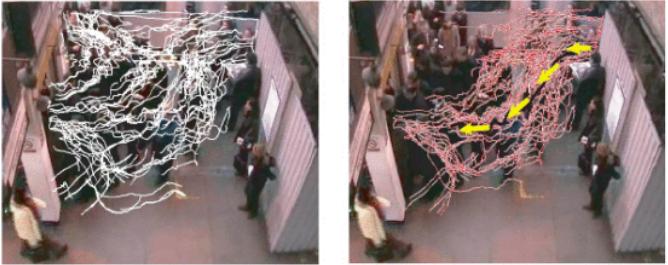
\includegraphics[width=0.6\textwidth]{dominantresult.png}
	\caption{Dominant motion detection results}
	\label{fig:dominantresult}
\end{figure}
By getting the trajectories of all the points, a new clustering framework Longest Common Subsequences (LCSS) is introduced. With the help of this framework, multiple trajectories are compared for the matching points and the dominant path is captured by clustering trajectories. The results of this model are shown in the figure \ref{fig:dominantresult}.
 